\section{Irvan Rizkiansyah/1174043}
	\subsection{Soal 1}
		\begin{itemize}
			\item Device Manager pada windows berfungsi untuk menampilkan segala macam perangkat hardware yang ter-inisialisasi oleh windows itu sendiri, dan juga berguna dalam mengelola perangkat hardware yang terpasang dan terdeteksi oleh windows.
			
			\item Direktori /dev pada linux pun berguna seperti device manager pada windows, dimana pada direktori /dev ini tersimpan konfigurasi perangkat device ataupun hardware yang terdeteksi oleh sistem.
			
		\end{itemize}
	\subsection{Soal 2}
	Langkah - langkah instalasi driver arduino :
		\begin{enumerate}
			\item Download terlebih dahulu driver arduino yang di sediakan di website arduino
			\item Kemudian hubungkan arduino ke PC, dan PC akan mendeteksi adanya perangkat yang terhubung namun tidak terbaca perangkat tersebut perangkat apa.
			\item Kemudian buka Device Manager
			\item Lalu pilih dan klik kanan pada perangkat arduino yg terdeteksi
			\item Kemudian pilih install driver atau update driver
			\item Nanti akan muncul pilihan mencari driver secara online atau mencari driver offline, pilih yang offline
			\item Cari file installer driver arduino yang sudah di download sebelumnya, kemudian pilih file installer driver arduino tersebut. dan akan langsung memulai peng-instal-an
			\item Tunggu hingga selesai dan pencet OK, maka driver arduino sudah ter-install
			
		\end{enumerate}
	\subsection{Soal 3}
	Di perlukan melakukan instalasi aplikasi arduino IDE untuk melihat dan mengecek baud rate dan port arduino kita yang terpasang, dengan memilih menu Tools kemudian pilih Serial monitor untuk melihat baud rate dan port dimana arduino yang terpasang.
	
	\subsection{Soal 4}
	Pada tahun 2002 PySerial pertama kalinya di luncurkan, dimana PySerial ini digunakan untuk berkomunikasi dengan mikrokontroller. Kemudian Library PySerial dikembangkan hingga sekarang.
	
	\subsection{Soal 5}
	Fungsi - fungsi yang ada pada PySerial :
		\begin{itemize}
			\item \begin{verbatim}open()\end{verbatim} 
			Berfungsi untuk membuka dan memberikan akses port serial yang terhubung
			\item \begin{verbatim}close()\end{verbatim} 
			Berfungsi untuk memberhentikan akses port serial yang terhubung
			\item \begin{verbatim}flush() \end{verbatim}
			Berfungsi untuk menghapus seluruh data yang ditampilkan, dan masih banyak yang lainnya.
			
		\end{itemize}
	
	\subsection{Soal 6}
	Dengan perulangan kita dapat melihat perkembangan dari mikrokontroller yang sedangn berjalan dari awal hingga akhir, apakah ada hal yang aneh, dengan perulangan semua data terbaca.
	Akan tetapi ada saat dimana perulangan tidak dibutuhkan, misalnya seperti kita hanya membutuhkan data hasil mikrokontroller yang berjalan pada saat tertentu saja, maka tanpa perulangan pun berguna.
	
	\subsection{Soal 7}
	Dalam membuat fungsi pada PySerial kita hanya perlua menginisialisasikan pembuatan fungsi seperti pada biasanya seperti : \begin{verbatim} def nama_fungsi() \end{verbatim}
	
	\subsection{Plagiarisme}
		\begin{figure}[ht]
            \centerline{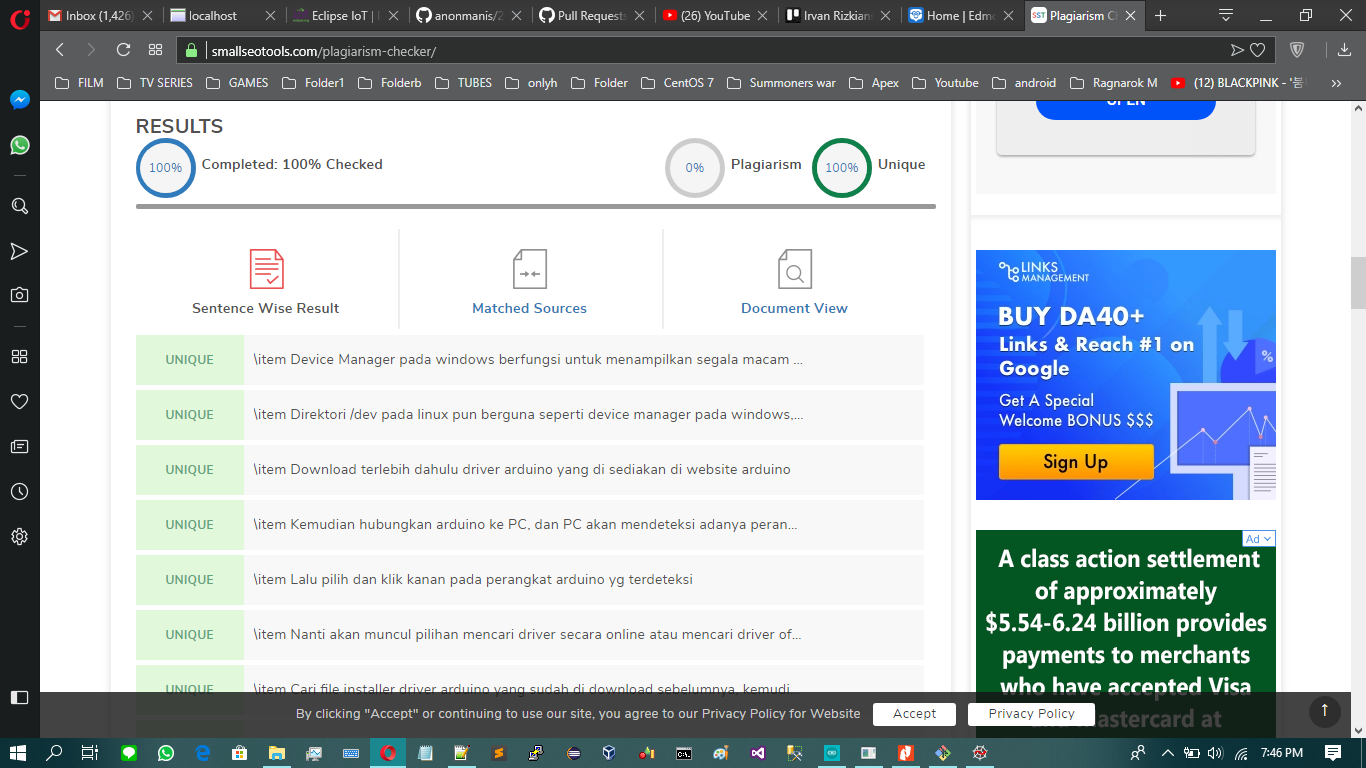
\includegraphics[width=0.5\textwidth]{figures/5/1174043/Teori/Plagiarisme.png}}
            \caption{Plagiarisme}
            \label{Plagiarisme}
        \end{figure}


\section{Hagan Rowlenstino/1174040}
	\subsection{Soal 1} 
		\begin{itemize}
			\item Device Manager : Seperti namanya sendiri, device manager berfungsi untuk menampilkan dan mengelola semua hardware yang terinstall ataupun dapat di instalasi ke dalam windows.

			\item folder /dev : Di dalam sistem operasi Linux, perangkat yang tehubung akan dianggap sebagai file. di dalam folder /dev inilah file - file  tersebut berada.
		\end{itemize}

	\subsection{Soal 2}
	Langkah - langkah instalasi driver arduino :
		\begin{enumerate}
			\item download file driver arduino terlebih dahulu dan masukkan ke dalam directory yang diinginkan
			\item hubungkan arduinio uno anda ke pc anda dengan kabel USB yang tersedia
			\item lalu windows akan memunculkan pop up yang memberitahu bahwa ingin menginstall dirver, tapi nanti tidak akan menemukan drivernya
			\item buka Device Manager 
			\item cari unknown device di dalam Device Manager di dalam tab other device
			\item klik kanan pada unknown device tersebut lalu pilih update driver software
			\item pilih browse my computer for driver software lalu masukkan directory dimana anda menyimpan driver arduino yang telah anda download tadi
			\item setelah itu klik install dan tunggu hingga proses selesai
			\item arduino pun sudah terbaca di pc anda 
		\end{enumerate}

	\subsection{Soal 3}
	Untuk melihat atau membaca baudrate dan port kita hanya perlu menginstall Arduino IDE, setelah itu buka menu serial monitor yang berada di tab tools. Dari sana akan terlihat baik baudrate dan port yang sedang digunakan oleh arduin anda.

	\subsection{Soal 4}
	PySerial merupakan sebuah library yang digunakan untuk komunikasi ke port serial terutama untuk mikrokontroller. PySerial pertama kali diluncurkan pada tahun 2002 yang makin berkembang dalam setiap versinya hingga tahun 2017 lalu.

	\subsection{Soal 5}
		\begin{itemize}
			\item \begin{verbatim}stop()\end{verbatim} : untuk menghentikan pembacaan program
			\item \begin{verbatim}serial.to_bytes(sequence)\end{verbatim} : berfungsi untuk mengubah sequence ke dalam bytes agar dapat dikirim ke dalam arduino.
			\item \begin{verbatim}close()\end{verbatim} : untuk menutup port dan menghentikan pembacaan program
		\end{itemize}

	\subsection{Soal 6}
	Dengan menggunakan pengulangan kita dapat mengambil data berkali - kali tanpa harus mengeksekusi file python tersebut berulang - ulang. Tanpa perulangan juga penting karena dapat digunakan di saat saat tertentu seperti jika ingin mengukur suhu ruangan yang hanya dilakukan pada saat saat tertentu tidak terus menerus.

	\subsection{Soal 7}
	Untuk membuat fungsi yang menggunakan pyserial kita hanya perlu untuk menginisialisasi pembubatan funsi dengan menggunakan def namafungsi() : lalu masukkan pyserial tersebut dengan indentasi. atau cukup dengan menggunakan fungsi while loop degan menggunakan while true:

	\subsection{Cek Plagiarisme}

	\begin{figure}
	[ht]
            \centerline{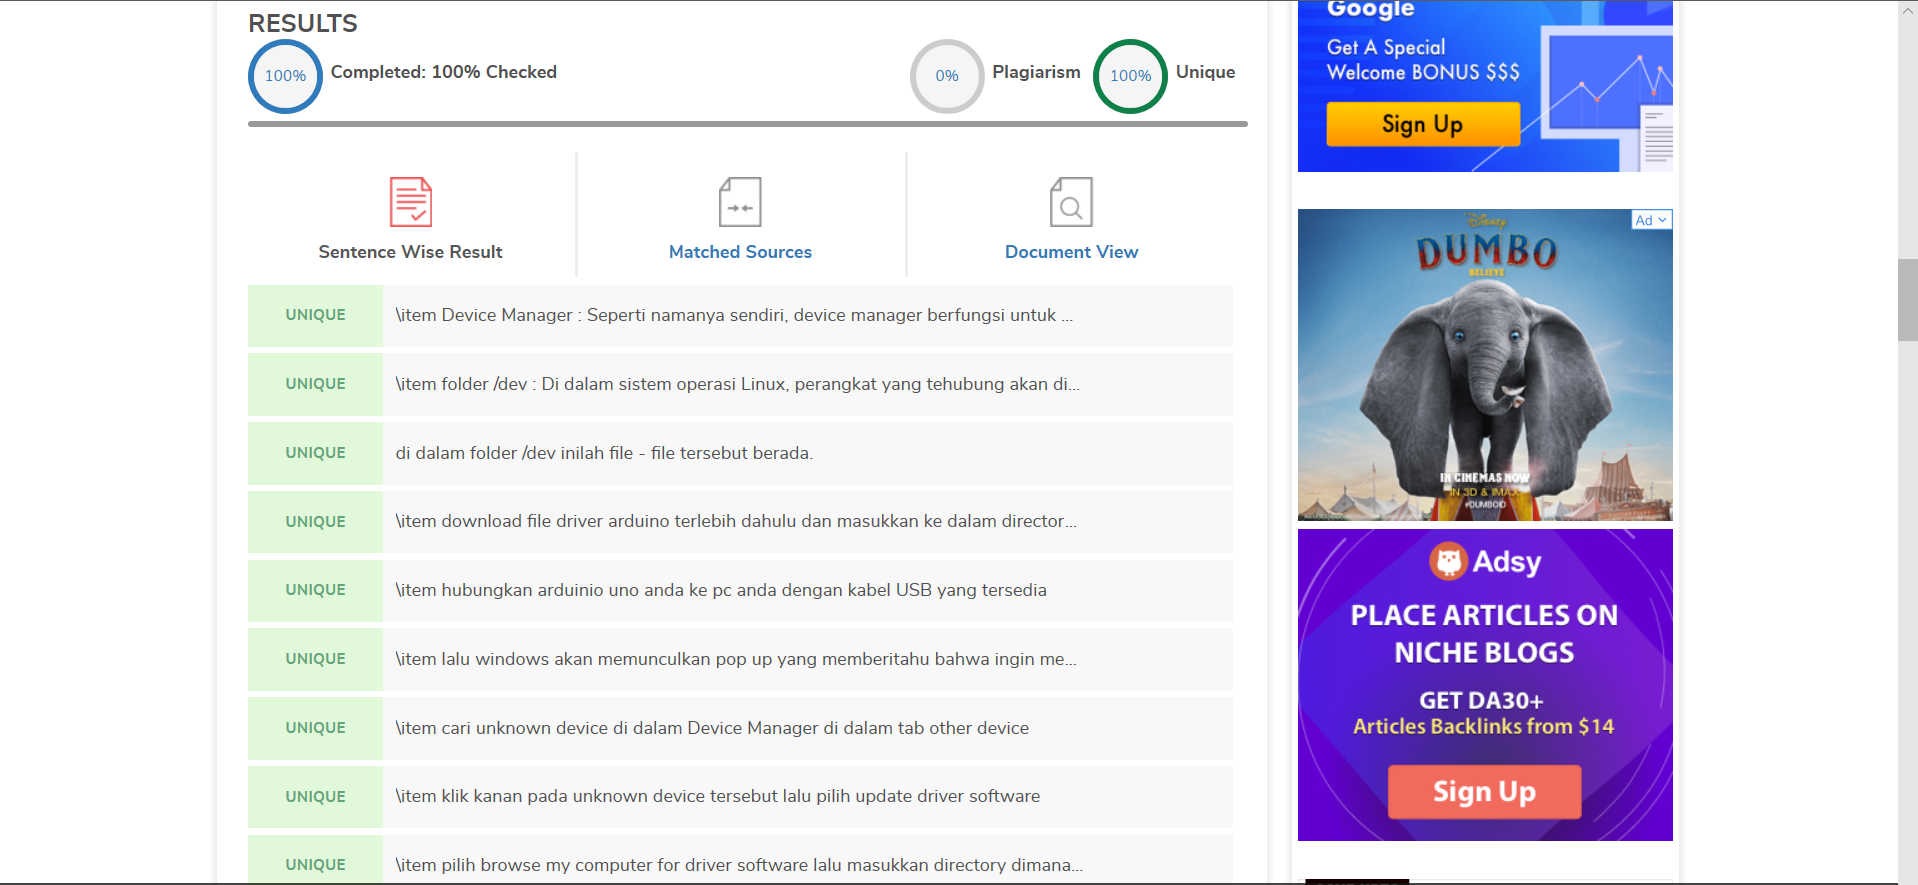
\includegraphics[width=0.5\textwidth]{figures/5/1174040/Teori/1174040_plagiat.png}}
            \caption{Cek Plagiarisme}
            \label{1174040_plagiat5}
            \end{figure}
    cek plagiarisme hagan
	

\section{Luthfi Muhammad Nabil/1174035}
\subsection{Soal 1}
Apa itu fungsi device manager di windows dan /dev di linux :
\begin{itemize}
	\item Device Manager merupakan panel kontrol pada sistem operasi windows. Pengguna dapat mengontrol dan melihat perangkat yang  telah terhubung dengan komputer dengan device manager. 
	Untuk setiap perangkat, pengguna dapat : 
		\begin{itemize}
			\item Memperbolehkan perangkat untuk beroperasi
			\item Menginformasikan sistem operasi untuk melakukan aksi pada perangkat yang tidak berfungsi
			\item Menginstall driver untuk perangkat yang terhubung
			\item Melihat informasi dari perangkat
		\end{itemize}
	\item /dev merupakan lokasi dari file untuk perangkat. /dev berfungsi untuk menampung data - data sebuah perangkat yang terhubung pada komputer. Perangkat yang dapat terhubung diantaranya perangkat penyimpanan data dan perangkat pengiriman data.
\end{itemize}

\subsection{Soal 2}
Jelaskan langkah - langkah instalasi driver dari arduino : 

Untuk instalasi driver, biasanya akan langsung terinstall jika sudah menginstall arduino IDE Seperti contoh meminta instalasi untuk arduino pada gambar \ref{PopUpInstalasi}.
\begin{figure} [ht]
		\centerline{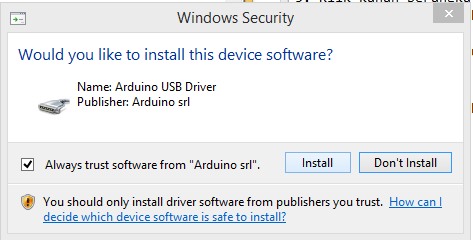
\includegraphics[width=1\textwidth]{figures/5/1174035/Teori/PopUpInstalasi.png}}
		\caption{Pop Up saat instalasi Arduino IDE}
		\label{PopUpInstalasi}
\end{figure}
Jika memang tidak ditemukan, maka ikuti langkah berikut : 
Yang dibutuhkan : 
\begin{itemize}
	\item Arduino Driver
	\item Arduino Jenis Apapun
\end{itemize}
Cara Instalasi : 
\begin{enumerate}
	\item Hubungkan arduino ke komputer (untuk arduino uno dapat menggunakan kabel type B)
	\begin{figure} [ht]
		\centerline{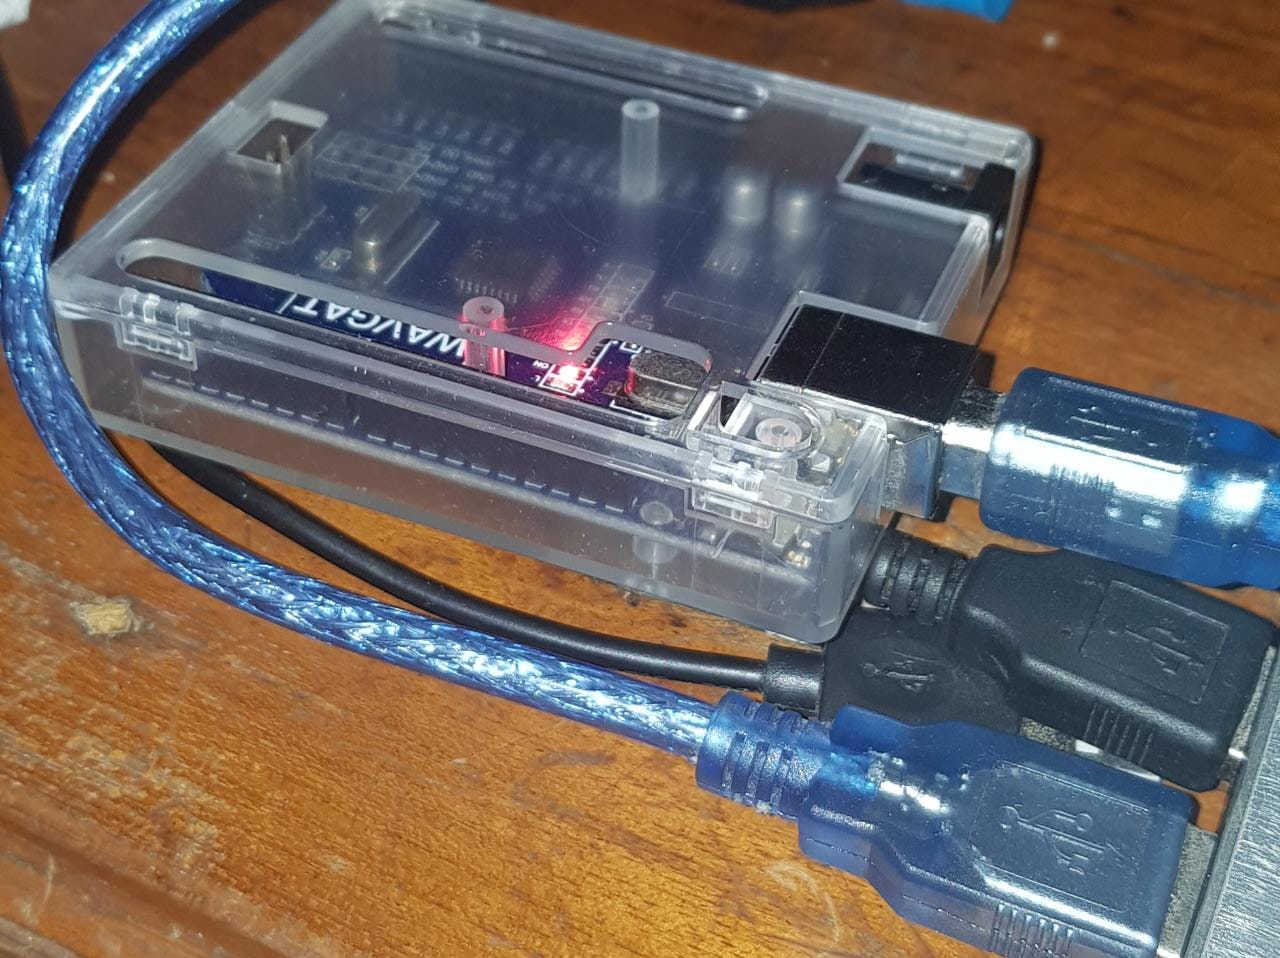
\includegraphics[width=0.6\textwidth]{figures/5/1174035/Teori/Soal1Step1.jpeg}}
		\caption{Hubungkan arduino dengan komputer}
		\label{Soal1Step1}
	\end{figure}
	\item Lalu setelah muncul popup instalasi driver akan terinstal secara otomatis. 
	\item Jika instalasi otomatis gagal, buka device manager.
		\begin{figure} [ht]
			\centerline{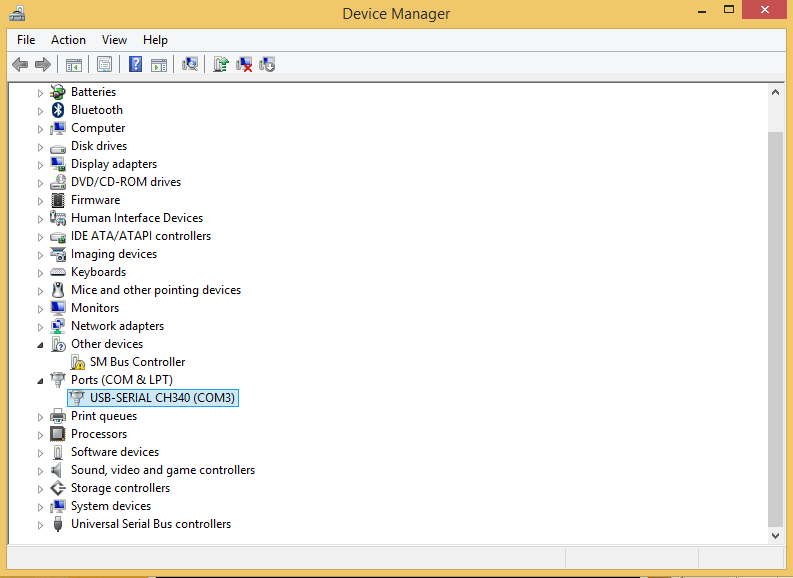
\includegraphics[width=1\textwidth]{figures/5/1174035/Teori/DeviceManagerContoh.png}}
			\caption{Tampilan Device Manager}
			\label{DevManagerContoh}
		\end{figure}
	\item Setelah device manager terbuka, cari perangkat lainnya/tidak diketahui (other device).
	\item Klik kanan perangkat yang tidak diketahui lalu pilih update driver.
	\item Pilih Cari driver (Browse my computer for driver software).
	\item Pilih lokasi driver ke driver yang telah didownload lalu klik next/ok.
	\item Setelah muncul pop up instalasi, tekan install.
	\item Instalasi Sukses
\end{enumerate}

\subsection{Soal 3}
Jelaskan bagaimana membaca baudrate dan port dari komputer yang sudah terinstall driver : 
\begin{itemize}
	\item Port : Untuk membaca port, dapat membuka file/lokasi berikut :
	
Arduino IDE : 
	\begin{figure} [ht]
			\centerline{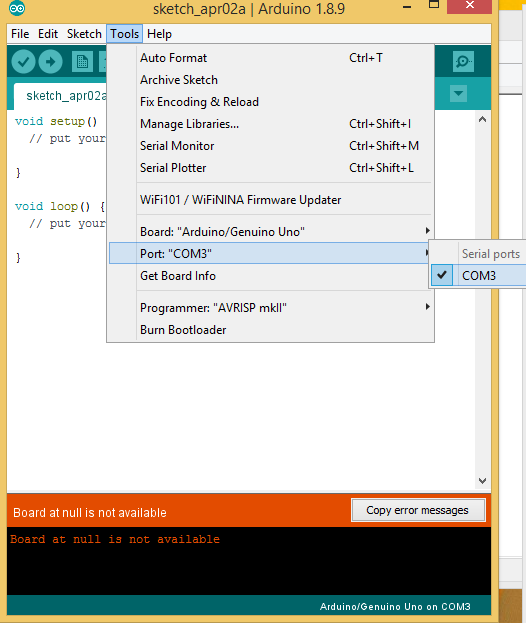
\includegraphics[width=0.6\textwidth]{figures/5/1174035/Teori/PortArduinoIDE.png}}
			\caption{Port dari Arduino IDE}
			\label{IDEPorts}
		\end{figure}
		\begin{enumerate}
			\item Buka Arduino IDE
			\item Lalu masuk ke Tools->Ports
			\item Akan muncul port serial untuk arduino seperti pada gambar \ref{IDEPorts}
		\end{enumerate}
Device Manager : 
	\begin{figure} [ht]
			\centerline{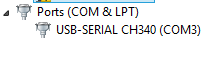
\includegraphics[width=0.6\textwidth]{figures/5/1174035/Teori/PortDeviceManager.png}}
			\caption{Port dari Device Manager}
			\label{DevManPort}
		\end{figure}
		\begin{enumerate}
			\item Buka Device Manager pada windows
			\item Cari Perangkat dengan nama Arduino
			\item Lalu lihat port berapa yang dipakai oleh Arduino Tersebut seperti pada gambar \ref{DevManPort}
		\end{enumerate}		
	\item Baudrate : Untuk melihat baudrate, dapat buka serial monitor dan cek baudrate dan tampilan fix pada tampilan serial monitor. Untuk setting default biasanya diantara 9600 dan 115200.
	\begin{figure} [ht]
			\centerline{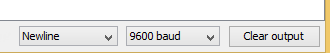
\includegraphics[width=0.6\textwidth]{figures/5/1174035/Teori/Baudrate.png}}
			\caption{Baud Rate}
			\label{BaudRate}
		\end{figure}
\end{itemize}

\subsection{Soal 4}
Sejarah PySerial : 

PySerial dibuat secara public pertama kali pada tahun 2002 dengan rilisan versi pertama 1.0. Pada saat itu PySerial sudah dapat membaca line serial dan menghapus semua isi dari serial tetapi belum dapat mengkonversi isi serial menjadi tipe data lain. PySerial juga sudah dapat melakukan Exception untuk proses yang terdapat error. Lalu pada tahun 2003 dirilis versi yang dapat mengkonversi data ke bilangan bulat, suppert terhadap python versi 2.2+ dan getter setter. Mulai pada tahun 2008, diberlakukan fitur iterasi untuk dapat mengambil seluruh data yang muncul pada serial yang diusulkan oleh Bernhard Bender. Kemudian pada tahun 2011, mulai dapat melihat daftar port yang terhubung dengan serial. Sampai akhirnya telah muncul versi 3.4 pada tahun 2017 yang sudah memperbaiki bug - bug yang ada.

\subsection{Soal 5}
Jelaskan fungsi - fungsi yang ada di pyserial.
\begin{itemize}
	\item \begin{verbatim}open()\end{verbatim} 
	Fungsi untuk membuka port serial yang terhubung
	\item \begin{verbatim}close()\end{verbatim} 
	Fungsi untuk menutup port serial yang terhubung
	\item \begin{verbatim}read(size=1) \end{verbatim}
	Fungsi untuk menentukan ukuran serial yang dapat dibaca
	\item \begin{verbatim}read\_until(expected=LF, size=None) \end{verbatim}
	Fungsi untuk membaca serial sampai sequence yang ditentukan sudah dapat.
	\item \begin{verbatim}write(data) \end{verbatim}
	Fungsi untuk menulis data ke perangkat yang terhubung.
	\item \begin{verbatim}flush() \end{verbatim}
	Fungsi untuk menghapus seluruh data yang ditampilkan di serial.
	\item \begin{verbatim}readline(size=-1) \end{verbatim}
	Untuk membaca setiap line pada tampilan yang ada pada serial
	\item \begin{verbatim}writelines(lines) \end{verbatim}
	Sama halnya dengan write yaitu untuk menulis data ke perangkat yang terhubung.
\end{itemize}
\subsection{Soal 6}
Jelaskan mengapa butuh perulangan dalam membaca serial : 

Karena perulangan digunakan untuk membaca seluruh data pada serial yang ada setiap baris. Perulangan digunakan agar data dapat muncul secara terus menerus atau realtime. Dalam konsep berjalannya sebuah microcontroller, proses yang ada akan dijalankan secara terus menerus sampai proses meminta atau processor meminta untuk memberhentikan proses tersebut sehingga jika tidak memakai perulangan, maka data yang diambil hanyalah data dimana sintaks untuk meminta data itu dipanggil. 
\subsection{Soal 7}
Jelaskan cara membuat fungsi yang menggunakan pyserial : 

Untuk membuat fungsi yang menggunakan pyserial, cukup dengan menuliskan fungsi dari pyserial dan menggunakannya dalam fungsi yang dibuat. Seperti contoh fungsi yang menggunakan PySerial : 
\lstinputlisting{src/5/1174035/Teori/chap5_1174035_teori.py}

\section{Faisal Najib Abdullah}
\subsection{Teori}
\begin{enumerate}
	\item Apa itu fungsi device manager di windows dan folder /dev di linux
	\par
		\begin{enumerate}
		    \item Device Manager : Seperti namanya sendiri, device manager berfungsi untuk menampilkan dan mengelola semua hardware yang terinstall ataupun dapat di instalasi ke dalam windows.

			\item folder /dev : Di dalam sistem operasi Linux, perangkat yang tehubung akan dianggap sebagai file. di dalam folder /dev inilah file - file  tersebut berada.
		\end{enumerate}
	
	\item Jelaskan langkah-langkah instalasi driver dari arduino
	\par
		Langkah - langkah instalasi driver arduino :
		\begin{enumerate}
			\item Pertama download file driver arduino terlebih dahulu dan masukkan ke dalam directory yang diinginkan.
			\item Hubungkan arduino uno anda ke pc anda dengan kabel USB yang tersedia.
			\item Kemudian windows akan memunculkan pop up yang memberitahu bahwa ingin menginstall dirver, tapi nanti tidak akan menemukan drivernya.
			\item Buka Device Manager dan cari unknown device di dalam Device Manager di dalam tab other device.
			\item Klik kanan pada unknown device tersebut lalu pilih update driver software
			\item Pilih browse my computer for driver software lalu masukkan directory dimana anda menyimpan driver arduino yang telah anda download tadi
			\item Setelah itu klik install dan tunggu hingga proses selesai
			\item Arduino pun sudah terbaca di pc anda 
		\end{enumerate}
	
	\item Jelaskan bagaimana cara membaca baudrate dan port dari komputer yang sudah terinstall driver
	\par
	Untuk melihat atau membaca baudrate dan port kita hanya perlu menginstall Arduino IDE, setelah itu buka menu serial monitor yang berada di tab tools. Dari sana akan terlihat baik baudrate dan port yang sedang digunakan oleh arduin anda.
	
	\item Jelaskan sejarah library pyserial
	\par
	PySerial merupakan sebuah library yang digunakan untuk komunikasi ke port serial terutama untuk mikrokontroller. PySerial pertama kali diluncurkan pada tahun 2002 yang makin berkembang dalam setiap versinya hingga tahun 2017 lalu.
	
	\item Jelaskan fungsi-fungsi apa saja yang dipakai dari library pyserial
		\begin{itemize}
			\item \begin{verbatim}serial.to_bytes(sequence)\end{verbatim} : berfungsi untuk mengubah sequence ke dalam bytes agar dapat dikirim ke dalam arduino.
			\item \begin{verbatim}stop()\end{verbatim} : untuk menghentikan pembacaan program
			\item \begin{verbatim}open()\end{verbatim} : Fungsi untuk membuka port serial yang terhubung
			\item \begin{verbatim}close()\end{verbatim} : Fungsi untuk menutup port serial yang terhubung
			\item \begin{verbatim}read(size=1) \end{verbatim} : Fungsi untuk menentukan ukuran serial yang dapat dibaca
			\item \begin{verbatim}close()\end{verbatim} : untuk menutup port dan menghentikan pembacaan program
		\end{itemize}
	
	\item Jelaskan kenapa butuh perulangan dalam tidak butuh perulangan dalam membaca serial
	\par
	Dengan menggunakan pengulangan kita dapat mengambil data berkali - kali tanpa harus mengeksekusi file python tersebut berulang - ulang. Tanpa perulangan juga penting karena dapat digunakan di saat saat tertentu seperti jika ingin mengukur suhu ruangan yang hanya dilakukan pada saat saat tertentu tidak terus menerus.
	
	\item Jelaskan bagaimana cara membuat fungsi yang mengunakan pyserial
	\par
	Untuk membuat fungsi yang menggunakan pyserial kita hanya perlu untuk menginisialisasi pembubatan funsi dengan menggunakan def namafungsi() : lalu masukkan pyserial tersebut dengan indentasi. atau cukup dengan menggunakan fungsi while loop degan menggunakan while true:
	
\end{enumerate}

\section{Ichsan Hizman Hardy}
{\Large \textbf{Teori}}
\subsection{Soal No. 1}
Apa itu fungsi device manager di windows dan folder /dev di linux?

\hfill \break
Fungsi device manager antara lain :
\begin{enumerate}
	\item Menunjukkan status suatu hardware.
	\item Menunjukkan informasi detil suatu hardware.
	\item Mengelola driver hardware
	\item Disable dan Enable hardware
	\item Mengidentifikasi konflik antar perangkat keras.
\end{enumerate}

\hfill \break
Folder /dev berisi file device, baik device blok maupun device karakter. Di dalamnya setodaknya ada file biner yang beernama MAKEDEV untuk membuat device secara manual.

\subsection{Soal No. 2}
Jelaskan langkah-langkah instalasi driver dari arduino!

\hfill \break
Berikut ini adalah langkah-langkah instalasi driver dari Arduino UNO di Windows:

\begin{enumerate}
	\item Hubungkan sistem minimun Arduino Uno ke komputer dengan kabel USB type B (kabel Printer).
	\item Lalu pada bagian kanan didesktop PC anda, akan muncul popup “Installing device driver software”.
	\item SIstem operasi Windows tidak menyediakan driver untuk Arduino Uno.
	\item Buka Device Manager, caranya pada bagian Search Program and Files lalu ketikkan “device manager” (tanpa tanda petik). Kemudian bagian Control Panel akan muncul halaman Device Manager, selanjutnya klik untuk menjalankan.
	\item Cari yang bernama Unknown device yang berada pada bagian Other device, biasanya ada tanda seru berwarna kuning, itu disebabkan karena penginstallan tidak berjalan dengan sempurna.
	\item Klik kanan pada “Unknown device” kemudian pilih Update Driver Software.
	\item Pilih Browse my computer for driver software.
	\item Arahkan lokasi folder ke folder ..arduino-1.0.5 drivers. Pastikan check-box lalu centang include subfolders. Klik Next untuk melanjutkan instalasi driver.
	\item Kemudian lanjutkan dengan mengklik Install pada tampilan Windows Security.
	\item Jika instalasi driver berhasil maka akan muncul Windows has successfully updated your driver software.
	\item Perhatikan dan ingat nama COM Arduino Uno, karena nama COM ini yang akan digunakan untuk meng-upload program nantinya.
\end{enumerate}

\subsection{Soal No. 3}
Jelaskan bagaimana cara membaca baudrate dan port dari komputer yang sudah terinstall driver!

\hfill \break
\textbf{Membaca Port dari Komputer}

\begin{enumerate}
	\item Hubungkan modul TX-RX serial dengan komputer melalui serial port menggunakan DB9 cable extension.
	\item Buka Hyper Terminal dengan menekan start kemudian All progams lalu Accessories kemudian Communications lalu Hyper Terminal.
	\item Ketik nama untuk Connection Description, misal coba, kemudian tekan OK.
	\item Pada Connect to, pilihlah COM port yang dipakai di Connect using, kemudian tekan OK.
	\item Masukkan nilai-nilai port settingnya, sesuai dengan DCE-nya. Kemudian tekan OK.
\end{enumerate}



\subsection{Soal No. 4}
Jelaskan sejarah library pyserial!

\hfill \break
PySerial adalah library/modul Python siap-pakai dan gratis yang dibuat untuk memudahkan kita dalam membuat program komunikasi data serial RS232 dalam bahasa Python.
Jika modul USB-2REL dapat kita kontrol dengan mudah menggunakan Python dan PyUSB (lihat pembahasannya di sini dan di sini), maka modul SER-2REL juga dapat kita kontrol dengan mudah menggunakan Python dengan bantuan modul PySerial.

\subsection{Soal No. 5}
Jelaskan fungsi-fungsi apa saja yang dipakai dari library pyserial!

\hfill \break
Fungsi-fungsi yang dipakai dari library PySerial, yaitu:
\begin{enumerate}
	\item Serial - fungsi ini untuk membuka port serial.
	\item write(data) - fungsi ini menulis data lewat port serial.
	\item readline() - fungsi ini membaca sebuah string dari port serial.
	\item read(size) - fungsi ini untuk membaca jumlah byte dari port serial.
	\item close() - fungsi ini untuk menutup port serial.
\end{enumerate}

\subsection{Soal No. 6}
Jelaskan kenapa butuh perulangan dan tidak butuh perulangan dalam membaca serial!

\hfill \break
Pada saat membaca serial di Arduino diperlukan perulangan agar bisa membaca data secara berulang kali sehingga data yang muncul banyak. Sedangkan apabila tidak membutuhkan perulangan maka Arduino hanya akan membaca data sekali saja.

\subsection{Soal No. 7}
Jelaskan bagaimana cara membuat fungsi yang mengunakan pyserial!

\hfill \break
Fungsi yang berada pada Python, dibuat dengan nama kata kunci def kemudian diikuti dengan nama fungsinya pada pyhton.
Seperti halnya dengan blok kode yang lain, kita juga harus memberikan identasi untuk menuliskan isi fungsi.

\section{Dika Sukma Pradana 1174050}
	\subsection{Pemahaman Teori}
		\begin{enumerate}
			\item Apa itu fungsi device manager di windows dan folder /dev di linux?
				\par
				Device manager merupakan perangkat lunak untuk menampilkan seluruh perangkat keras yang di-inisialisasi atau dikenali oleh sistem operasi Windows. Device Manager membantu dalam mengelola atau me-manage semua perangkat keras yang terpasang dan terdeteksi dalam sistem Windows. Perangkat keras tersebut bisa berupa harddisk, kartu VGA, sound, keyboard, perangkat USB dan lain-lainnya.
				
				\par
				Fungsi device manager antara lain :
					\begin{itemize}
						\item Menunjukkan status mengenai suatu perangkat keras.
						\item Menunjukkan informasi detail mengenai suatu perangkat keras.
						\item Mengelola driver perangkat keras.
						\item Menonaktifkan dan mengaktifkan perangkat keras.
						\item Mengidentifikasi konflik antar perangkat keras.
						\item Memberitahukan terjadinya masalah pada perangkat keras.
					\end{itemize}

				\par
				Folder /dev merupakan representasi dari drive yang terhubung ke sistem operasi Linux dan oleh sistem dianggap sebagai file-file direktori. Biasanya sering ditampilkan direktori seperti /dev/sda1 yang mewakili Drive SATA pertama dalam sistem.
				
			\item Jelaskan langkah-langkah instalasi driver dari arduino!
				\begin{enumerate}
					\item Hubungkan sistem minimun Arduino Uno ke komputer dengan kabel USB type B (kabel Printer).
					\item Lalu pada bagian kanan didesktop PC anda, akan muncul popup Installing device driver software seperti pada gambar dibawah ini.
					\item Windows tidak menyediakan driver arduino, jadi kita harus menginstal secara manual.
					\item Buka Device Manager, klik untuk menjalankan.
					\item Cari Unknown device pada bagian Other device, bila terdapat tanda seru berarti peroses penginstalan belum berhasil sepenuhnya.
					\item Klik kanan pada Unknown device lalu pilih Update Driver Software.
					\item Pilih Browse my computer for driver software.
					\item Arahkan lokasi folder ke folder ..arduino1.0.5 drivers. Pastikan checkbox lalu centang include subfolders. Klik Next untuk melanjutkan instalasi driver.
					\item Kemudian lanjutkan dengan mengklik Install pada tampilan Windows Security.
					\item Jika instalasi driver berhasil maka akan muncul Windows has successfully updated your driver software.
					\item Perhatikan dan ingat nama COM Arduino Uno, karena nama COM ini yang akan digunakan untuk meng-upload program nantinya.
				\end{enumerate}
				
			\item Jelaskan bagaimana cara membaca baudrate dan port dari komputer yang sudah terinstall driver!
				\begin{itemize}
					\item Membaca Baudrate dari Komputer
						\begin{enumerate}
							\item Pertama buka Start. Cari Device Manager, lalu klik.
							\item Kemudian pilih Ports (COM \& LPT).
							\item Klik dua kali pada COM yang terhubung.
							\item Pilih tab Port Settings, lalu lihat di Bit per second.
						\end{enumerate}
					\item Membaca Port dari Komputer
						\begin{enumerate}
							\item Pertama buka Start. Cari Device Manager, lalu klik.
							\item Kemudian pilih Ports (COM \& LPT).
							\item Port dari Arduino telah terbaca oleh PC.
						\end{enumerate}
				\end{itemize}
							
			\item Jelaskan sejarah library pyserial!
			\par 
			PySerial adalah paket Python yang menfasilitasi komunikasi serial antara PC dengan perangkat keras eksternal. PySerial menyediakan antarmuka untuk berkomunikasi melalui protokol komunikasi serial. Komunikasi serial adalah salah satu protokol komunikasi komputer tertua. Protokol komunikasi serial mendahului spesifikasi USB yang digunakan oleh komputer dan perangkat keras lain seperti mouse, keyboard, dan webcam. USB adalah singkatan dari Universal Serial Bus. USB dan dibangun di atas dan memperluas antarmuka komunikasi serial asli.
			
			\item Jelaskan fungsi-fungsi apa saja yang dipakai dari library pyserial!
			Fungsi-fungsi yang dipakai dari library PySerial, yaitu:
				\begin{itemize}
					\item \begin{verbatim} serial \end{verbatim} : fungsi ini untuk membuka port serial.
					\item \begin{verbatim} write(data) \end{verbatim} : fungsi ini menulis data lewat port serial.
					\item \begin{verbatim} readline() \end{verbatim} : fungsi ini membaca sebuah string dari port serial.
					\item \begin{verbatim} read(size) \end{verbatim} fungsi ini untuk membaca jumlah byte dari port serial.
					\item \begin{verbatim} close() \end{verbatim} : fungsi ini untuk menutup port serial.
				\end{itemize}
			
			\item Jelaskan kenapa butuh perulangan dan tidak butuh perulangan dalam membaca serial!
			\par
			Perualangan dalam bahasa pemrograman berfungsi menyuruh komputer melakukan sesuatu secara berulang-ulang. Terdapat dua jenis perualangan dalam bahasa pemrograman python, yaitu perulangan dengan for dan while. Perulangan for disebut counted loop (perulangan yang terhitung), sementara perulangan while disebut uncounted loop (perulangan yang tak terhitung). Perulangan for biasanya digunakan untuk mengulangi kode yang sudah dipastikan banyak perulangannya. Sedangkan while untuk perulangan yang ditentukan dan belum pasti banyaknya. Perulangan diperlukan agar dapat membaca data secara berulang kali sehingga data yang muncul lebih dari satu.  Sedangkan apabila tidak memakai perulangan maka data akan terbaca satu kali saja.
			
			\item Jelaskan bagaimana cara membuat fungsi yang mengunakan pyserial!
				\begin{verbatim}			
					import serial

					def baca():
						ser = serial.Serial("COM4",9600)
						baca = ser.readline()
						print(baca)

					baca()
				\end{verbatim}
				
			\item Plagiarism
			\begin{figure}[H]
				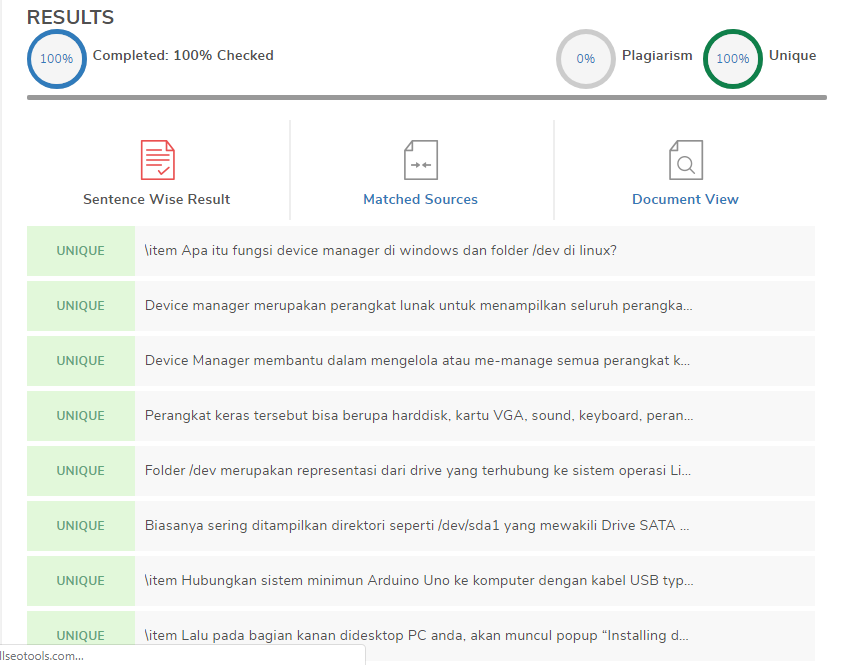
\includegraphics[width=10cm]{figures/5/1174050/Teori/plagiarism.png}
				\centering
				\caption{Hasil Scan Plagiarism}
			\end{figure}
			
		\end{enumerate}